\documentclass{article}
\usepackage{graphicx}
\usepackage[margin=1.5cm]{geometry}
\usepackage{amsmath}

\begin{document}

\title{Warm Up Activity: Unit 6, Momentum}
\author{Prof. Jordan C. Hanson}

\maketitle

\section{Memory Bank}

\begin{itemize}
\item $\vec{p} = m \vec{v}$ ... Definition of momentum.
\item $\vec{p}_f = \vec{p}_i$ ... Momentum conservation: no net forces.
\end{itemize}

\section{Momentum}

\begin{enumerate}
\item A gas molecule has a mass of $20 \times 10^{-25}$ kg and an average speed of 350 m/s.  What is the momentum in kg m/s? \\ \vspace{1cm}
\begin{figure}[ht]
\centering
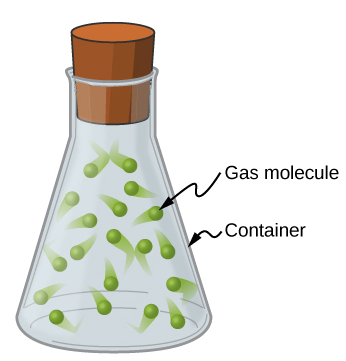
\includegraphics[width=0.3\textwidth]{gas.png}
\caption{\label{fig:gas} A beaker full of gas molecules.}
\end{figure}
\item Suppose this molecule collides with the side of the glass beaker, turns around, and flies off in exactly the opposite direction at the same speed.  What is the \textit{change} in momentum, $\Delta \vec{p} = \vec{p}_f - \vec{p}_i$?  (This is how we build up the \textbf{kinetic theory of gases} in Physics 3...stay tuned). \\ \vspace{1cm}
\end{enumerate}

\section{Momentum Conservation}
\begin{enumerate}
\item Two molecules collide and stick together, forming one larger molecule.  Each molecule weighs $20 \times 10^{-25}$ kg.  One has a velocity of 350 m/s, and the other has a velocity of -350 m/s.  (a) What is the total initial momentum (adding the two momenta)? (b) What is the final speed of the big new molecule?
\end{enumerate}

\end{document}